\documentclass[12pt, xcolor=table]{beamer}
\usepackage{graphicx}
\usepackage[ngerman]{babel}
\usepackage[utf8]{inputenc}
\usepackage{amsmath}
\usepackage{amssymb}
\usepackage{listings}
\usepackage{hyperref}
\usepackage{fancyvrb}
\usepackage{color}
\usepackage{alltt}

\usepackage[percent]{overpic}
\usepackage[footnotesize, bf]{caption}
%Copyright 2008 by Adrian Böhmichen
%
% This file is free software: you can redistribute it and/or modify
% it under the terms of the GNU General Public License as published by
% the Free Software Foundation, either version 3 of the License, or
% (at your option) any later version.
%
% This file is distributed in the hope that it will be useful,
% but WITHOUT ANY WARRANTY; without even the implied warranty of
% MERCHANTABILITY or FITNESS FOR A PARTICULAR PURPOSE.  See the
% GNU General Public License for more details.
%
% You should have received a copy of the GNU General Public License
% along with this file.  If not, see <http://www.gnu.org/licenses/>.

%%%%%%%%%%%%%%%%%%%%%%%%%%%%%%%%%%%%%%%%%%%%%%%%%%%%%%%%%%%%%%%%%
%     Ubuntuusers Vorlage für ein LaTeX-Beamer Theme            %
%                                                               %
% Für das Korrekte funktionieren benötigt man einen header.png  %
% und ein logo.png Datei!                                       %
% Zusätzlich muss man folgende Pakete benutzten:                %
%   \usepackage{graphicx}                                       %
%   \usepackage[percent]{overpic}                               %
%                                                               %
% Danach muss nur noch am Anfang die Datei                      %
% mit \input{} eingebunden werden.                              %
%                                                               %
%%%%%%%%%%%%%%%%%%%%%%%%%%%%%%%%%%%%%%%%%%%%%%%%%%%%%%%%%%%%%%%%%

%weitere Farbe spezifizieren:
%Farben von dem Humantheme
%\definecolor{Orange}{RGB}{240,165,19}
\definecolor{Orange}{RGB}{5,215,242}
%\definecolor{Human-Base}{RGB}{129,102,71}
\definecolor{Human-Base}{RGB}{5,25,242}
%Farben aus dem Inyokatheme
%\definecolor{uuheader1}{RGB}{164,143,101}
\definecolor{uuheader1}{RGB}{5,25,242}
%\definecolor{uuheader2}{RGB}{129,106,59}
\definecolor{uuheader2}{RGB}{5,25,242}


%Theme festlegen für alle Templates die nicht selbstständig definiert werden:
\usepackage{beamerthemedefault}


%Definieren des Innertheme, zuständig für die Symbole bei Listen
\setbeamertemplate{sections/subsections in toc}[square]
\setbeamertemplate{items}[circle]

\setbeamercolor{item}{fg=Human-Base}

%entfernen der Navigationsleiste
\beamertemplatenavigationsymbolsempty

%Logo definieren, man kann die Lage nicht verändern
%\logo{\includegraphics[scale=0.1]{logo.png}}


%Kopf- und Fußzeile definieren
%\setbeamertemplate{headline}
%{%
%\begin{overpic}[width=\paperwidth
% nächste Zeile dient zum anzeigen eines Rasters, für das paltzieren des ToC hilfreich
%,grid,tics=10
%]
%{header.png}%
%  \put(0,11){\insertsectionnavigationhorizontal{\paperwidth}{~}{~}}%
%  \end{overpic}
%}

\setbeamertemplate{footline}[text line]
{%
\begin{minipage}[b]{116mm}
\insertauthor \hfill%
%neue Navigationsleiste
 \insertframenumber ~/ \inserttotalframenumber\\[1ex]
\end{minipage}
}

% Farben festlegen ausserhalb des innertheme

%Allgemeine Angaben und Verbesserung vom default Theme
\setbeamercolor{structure}{fg=uuheader1}
\setbeamercolor{section in toc}{fg=Human-Base}
\setbeamercolor{subsection in toc}{parent=section in toc}
\setbeamercolor{framesubtitle}{fg=uuheader2}


%Farbe und Form der Blöcke definieren
\setbeamertemplate{blocks}[rounded]
%\setbeamercolor{block title}{fg=uuheader1,bg=Orange}
%\setbeamercolor{block title alerted}{use=alerted text,fg=black,bg=alerted text.fg!75!bg}
%\setbeamercolor{block title example}{use=example text,fg=black,bg=example text.fg!75!bg}

%\setbeamercolor{block body}{parent=normal text,use=block title,bg=block title.bg!25!bg}
%\setbeamercolor{block body alerted}{parent=normal text,use=block title alerted,bg=block title alerted.bg!25!bg}
%\setbeamercolor{block body example}{parent=normal text,use=block title example,bg=block title example.bg!25!bg}

%Für den Titleframe
\setbeamertemplate{title page}[default][rounded=true]
\setbeamercolor{title}{fg=uuheader2,bg=Orange}


\makeatletter
\def\PY@reset{\let\PY@it=\relax \let\PY@bf=\relax%
    \let\PY@ul=\relax \let\PY@tc=\relax%
    \let\PY@bc=\relax \let\PY@ff=\relax}
\def\PY@tok#1{\csname PY@tok@#1\endcsname}
\def\PY@toks#1+{\ifx\relax#1\empty\else%
    \PY@tok{#1}\expandafter\PY@toks\fi}
\def\PY@do#1{\PY@bc{\PY@tc{\PY@ul{%
    \PY@it{\PY@bf{\PY@ff{#1}}}}}}}
\def\PY#1#2{\PY@reset\PY@toks#1+\relax+\PY@do{#2}}

\def\PY@tok@gd{\def\PY@tc##1{\textcolor[rgb]{0.63,0.00,0.00}{##1}}}
\def\PY@tok@gu{\let\PY@bf=\textbf\def\PY@tc##1{\textcolor[rgb]{0.50,0.00,0.50}{##1}}}
\def\PY@tok@gt{\def\PY@tc##1{\textcolor[rgb]{0.00,0.25,0.82}{##1}}}
\def\PY@tok@gs{\let\PY@bf=\textbf}
\def\PY@tok@gr{\def\PY@tc##1{\textcolor[rgb]{1.00,0.00,0.00}{##1}}}
\def\PY@tok@cm{\let\PY@it=\textit\def\PY@tc##1{\textcolor[rgb]{0.25,0.50,0.50}{##1}}}
\def\PY@tok@vg{\def\PY@tc##1{\textcolor[rgb]{0.10,0.09,0.49}{##1}}}
\def\PY@tok@m{\def\PY@tc##1{\textcolor[rgb]{0.40,0.40,0.40}{##1}}}
\def\PY@tok@mh{\def\PY@tc##1{\textcolor[rgb]{0.40,0.40,0.40}{##1}}}
\def\PY@tok@go{\def\PY@tc##1{\textcolor[rgb]{0.50,0.50,0.50}{##1}}}
\def\PY@tok@ge{\let\PY@it=\textit}
\def\PY@tok@vc{\def\PY@tc##1{\textcolor[rgb]{0.10,0.09,0.49}{##1}}}
\def\PY@tok@il{\def\PY@tc##1{\textcolor[rgb]{0.40,0.40,0.40}{##1}}}
\def\PY@tok@cs{\let\PY@it=\textit\def\PY@tc##1{\textcolor[rgb]{0.25,0.50,0.50}{##1}}}
\def\PY@tok@cp{\def\PY@tc##1{\textcolor[rgb]{0.74,0.48,0.00}{##1}}}
\def\PY@tok@gi{\def\PY@tc##1{\textcolor[rgb]{0.00,0.63,0.00}{##1}}}
\def\PY@tok@gh{\let\PY@bf=\textbf\def\PY@tc##1{\textcolor[rgb]{0.00,0.00,0.50}{##1}}}
\def\PY@tok@ni{\let\PY@bf=\textbf\def\PY@tc##1{\textcolor[rgb]{0.60,0.60,0.60}{##1}}}
\def\PY@tok@nl{\def\PY@tc##1{\textcolor[rgb]{0.63,0.63,0.00}{##1}}}
\def\PY@tok@nn{\let\PY@bf=\textbf\def\PY@tc##1{\textcolor[rgb]{0.00,0.00,1.00}{##1}}}
\def\PY@tok@no{\def\PY@tc##1{\textcolor[rgb]{0.53,0.00,0.00}{##1}}}
\def\PY@tok@na{\def\PY@tc##1{\textcolor[rgb]{0.49,0.56,0.16}{##1}}}
\def\PY@tok@nb{\def\PY@tc##1{\textcolor[rgb]{0.00,0.50,0.00}{##1}}}
\def\PY@tok@nc{\let\PY@bf=\textbf\def\PY@tc##1{\textcolor[rgb]{0.00,0.00,1.00}{##1}}}
\def\PY@tok@nd{\def\PY@tc##1{\textcolor[rgb]{0.67,0.13,1.00}{##1}}}
\def\PY@tok@ne{\let\PY@bf=\textbf\def\PY@tc##1{\textcolor[rgb]{0.82,0.25,0.23}{##1}}}
\def\PY@tok@nf{\def\PY@tc##1{\textcolor[rgb]{0.00,0.00,1.00}{##1}}}
\def\PY@tok@si{\let\PY@bf=\textbf\def\PY@tc##1{\textcolor[rgb]{0.73,0.40,0.53}{##1}}}
\def\PY@tok@s2{\def\PY@tc##1{\textcolor[rgb]{0.73,0.13,0.13}{##1}}}
\def\PY@tok@vi{\def\PY@tc##1{\textcolor[rgb]{0.10,0.09,0.49}{##1}}}
\def\PY@tok@nt{\let\PY@bf=\textbf\def\PY@tc##1{\textcolor[rgb]{0.00,0.50,0.00}{##1}}}
\def\PY@tok@nv{\def\PY@tc##1{\textcolor[rgb]{0.10,0.09,0.49}{##1}}}
\def\PY@tok@s1{\def\PY@tc##1{\textcolor[rgb]{0.73,0.13,0.13}{##1}}}
\def\PY@tok@sh{\def\PY@tc##1{\textcolor[rgb]{0.73,0.13,0.13}{##1}}}
\def\PY@tok@sc{\def\PY@tc##1{\textcolor[rgb]{0.73,0.13,0.13}{##1}}}
\def\PY@tok@sx{\def\PY@tc##1{\textcolor[rgb]{0.00,0.50,0.00}{##1}}}
\def\PY@tok@bp{\def\PY@tc##1{\textcolor[rgb]{0.00,0.50,0.00}{##1}}}
\def\PY@tok@c1{\let\PY@it=\textit\def\PY@tc##1{\textcolor[rgb]{0.25,0.50,0.50}{##1}}}
\def\PY@tok@kc{\let\PY@bf=\textbf\def\PY@tc##1{\textcolor[rgb]{0.00,0.50,0.00}{##1}}}
\def\PY@tok@c{\let\PY@it=\textit\def\PY@tc##1{\textcolor[rgb]{0.25,0.50,0.50}{##1}}}
\def\PY@tok@mf{\def\PY@tc##1{\textcolor[rgb]{0.40,0.40,0.40}{##1}}}
\def\PY@tok@err{\def\PY@bc##1{\fcolorbox[rgb]{1.00,0.00,0.00}{1,1,1}{##1}}}
\def\PY@tok@kd{\let\PY@bf=\textbf\def\PY@tc##1{\textcolor[rgb]{0.00,0.50,0.00}{##1}}}
\def\PY@tok@ss{\def\PY@tc##1{\textcolor[rgb]{0.10,0.09,0.49}{##1}}}
\def\PY@tok@sr{\def\PY@tc##1{\textcolor[rgb]{0.73,0.40,0.53}{##1}}}
\def\PY@tok@mo{\def\PY@tc##1{\textcolor[rgb]{0.40,0.40,0.40}{##1}}}
\def\PY@tok@kn{\let\PY@bf=\textbf\def\PY@tc##1{\textcolor[rgb]{0.00,0.50,0.00}{##1}}}
\def\PY@tok@mi{\def\PY@tc##1{\textcolor[rgb]{0.40,0.40,0.40}{##1}}}
\def\PY@tok@gp{\let\PY@bf=\textbf\def\PY@tc##1{\textcolor[rgb]{0.00,0.00,0.50}{##1}}}
\def\PY@tok@o{\def\PY@tc##1{\textcolor[rgb]{0.40,0.40,0.40}{##1}}}
\def\PY@tok@kr{\let\PY@bf=\textbf\def\PY@tc##1{\textcolor[rgb]{0.00,0.50,0.00}{##1}}}
\def\PY@tok@s{\def\PY@tc##1{\textcolor[rgb]{0.73,0.13,0.13}{##1}}}
\def\PY@tok@kp{\def\PY@tc##1{\textcolor[rgb]{0.00,0.50,0.00}{##1}}}
\def\PY@tok@w{\def\PY@tc##1{\textcolor[rgb]{0.73,0.73,0.73}{##1}}}
\def\PY@tok@kt{\def\PY@tc##1{\textcolor[rgb]{0.69,0.00,0.25}{##1}}}
\def\PY@tok@ow{\let\PY@bf=\textbf\def\PY@tc##1{\textcolor[rgb]{0.67,0.13,1.00}{##1}}}
\def\PY@tok@sb{\def\PY@tc##1{\textcolor[rgb]{0.73,0.13,0.13}{##1}}}
\def\PY@tok@k{\let\PY@bf=\textbf\def\PY@tc##1{\textcolor[rgb]{0.00,0.50,0.00}{##1}}}
\def\PY@tok@se{\let\PY@bf=\textbf\def\PY@tc##1{\textcolor[rgb]{0.73,0.40,0.13}{##1}}}
\def\PY@tok@sd{\let\PY@it=\textit\def\PY@tc##1{\textcolor[rgb]{0.73,0.13,0.13}{##1}}}

\def\PYZbs{\char`\\}
\def\PYZus{\char`\_}
\def\PYZob{\char`\{}
\def\PYZcb{\char`\}}
\def\PYZca{\char`\^}
\def\PYZsh{\char`\#}
\def\PYZpc{\char`\%}
\def\PYZdl{\char`\$}
\def\PYZti{\char`\~}
% for compatibility with earlier versions
\def\PYZat{@}
\def\PYZlb{[}
\def\PYZrb{]}
\makeatother

\renewcommand{\footnotesize}{\tiny}
\begin{document}
\title{Algorithmen und Analyse auf bibliographischen Daten}
\author{peterr und Lusy}
\date{\today}

\begin{frame}
	\titlepage
\end{frame}

\begin{frame}
	\frametitle{Eigenschaften des Datensatzes}
	\begin{itemize}
		\item  enthält ca. $706\,000$ Einträge
		\item  mit 19 verschiedenen Themengebieten
		\item  nur der Themenbereich Physik wird in Themengruppen unterteilt
		\item  11 Einträge ohne Informationen
		\item  Publikationen haben im Durchschnitt 1.3 und maximal 9 Themen
	\end{itemize}
\end{frame}

\begin{frame}
	\frametitle{Verteilung der Themen}
	\begin{center}
		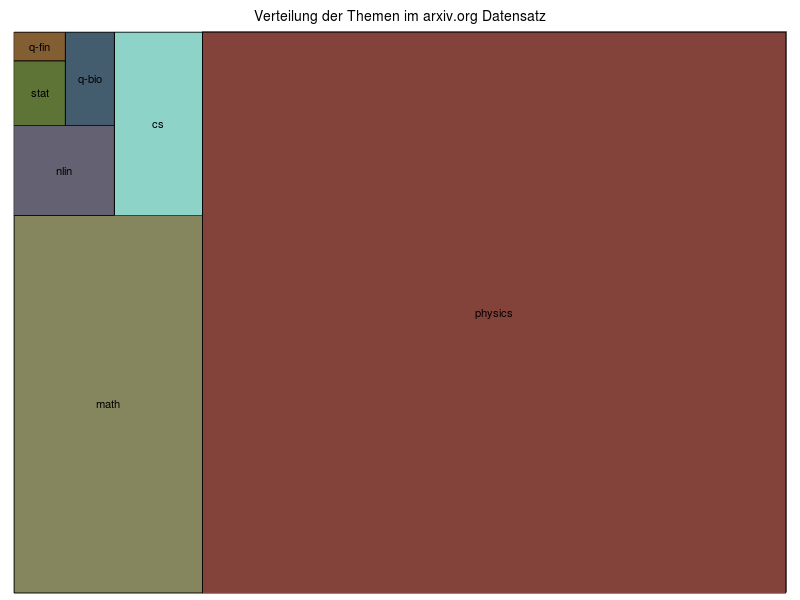
\includegraphics[scale=0.35]{../../visual/treeParent2.png}
	\end{center}
\end{frame}

\begin{frame}[fragile]
    \frametitle{Verteilung der Themen in Computer Science}
    \begin{block}{Subjects in CS: Summary}
    	\begin{alltt}\tiny
most frequent items:
                  Computer Science - Information Theory
                                                   6646
             Computer Science - Artificial Intelligence
                                                   3045
      Computer Science - Data Structures and Algorithms
                                                   2878
Computer Science - Networking and Internet Architecture
                                                   2660
           Computer Science - Logic in Computer Science
                                                   2498
                                                (Other)
                                                  58364

element (itemset/transaction) length distribution:
sizes
    1     2     3     4     5     6     7     8     9    10    11    12    13
13906  9209  5443  2802  1351   684   317   173    73    41    16    15     7
   14    15    16    17    19    21    22
    6     5     1     1     1     1     1

   Min. 1st Qu.  Median    Mean 3rd Qu.    Max.
  1.000   1.000   2.000   2.234   3.000  22.000

\end{alltt}

	\end{block}
\end{frame}

\begin{frame}
	\frametitle{Verteilung der Themen in Computer Science}
	\begin{center}
		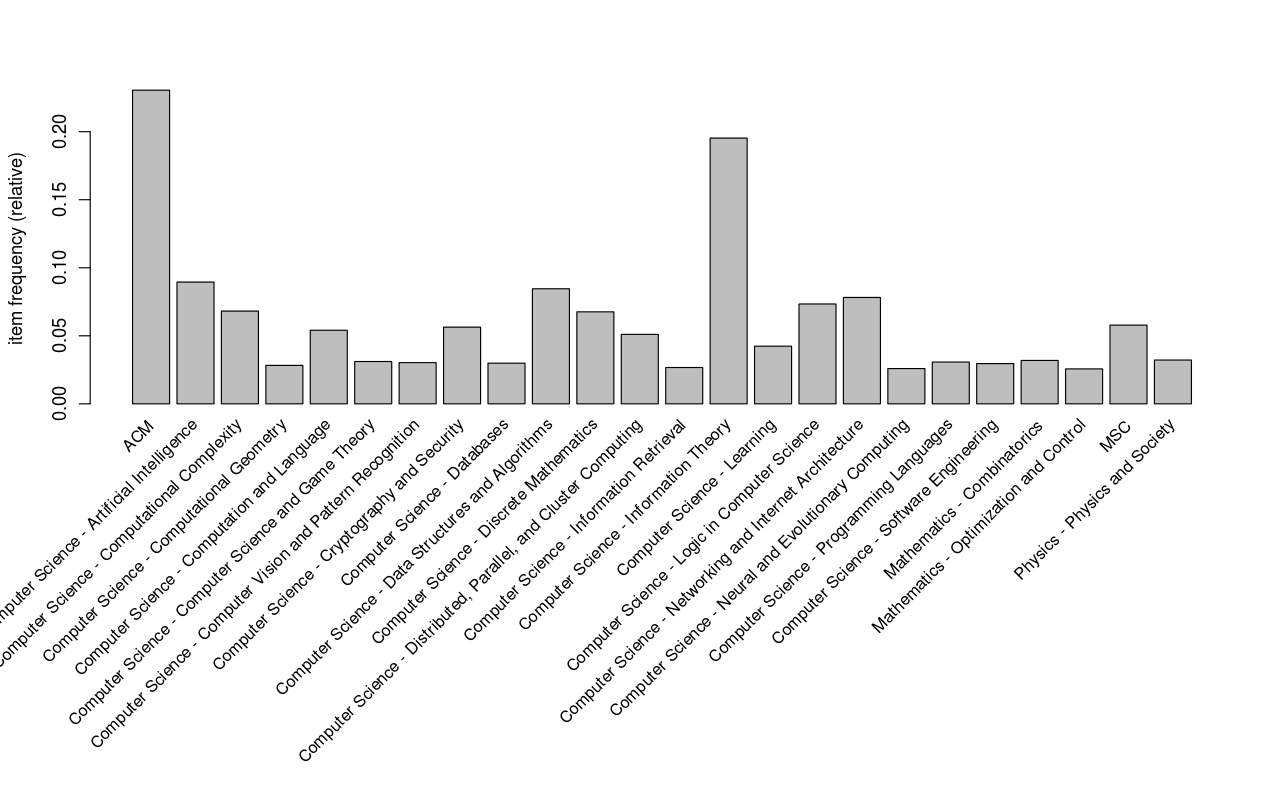
\includegraphics[scale=0.25]{../../visual/csFrequent_filter_acm_and_msc.png}
	\end{center}
\end{frame}
\begin{frame}
	\frametitle{Verteilung der Themen in Computer Science}
    VOSviewer demo
	\begin{center}
		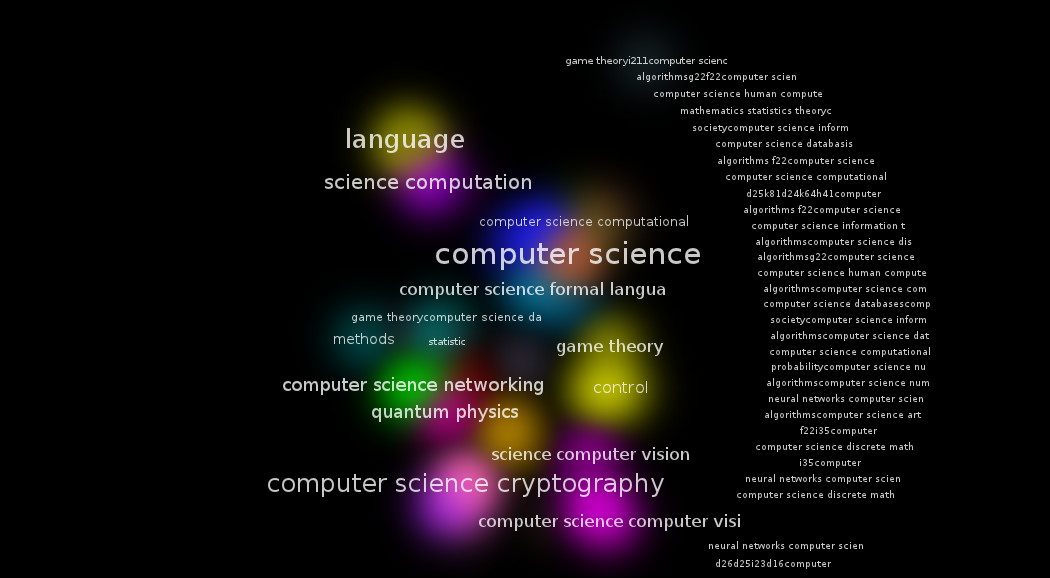
\includegraphics[scale=0.25]{../../visual/cs_subs_cluster_density.png}
	\end{center}
\end{frame}
\begin{frame}
	\frametitle{Entwicklung über die Zeit}
\end{frame}
\begin{frame}
	\frametitle{Interpretation der Ergebnisse}
    \begin{block}{Assoziationsregeln - Kenngrößen}
    \begin{center}
        \begin{itemize}
			\item Support - relative Häufigkeit der Menge in den Daten
			\item Konfidenz - Häufikeit des gemeinsames Auftretens von A und B, unter der Bedingung das A auftritt
			\item Lift - Bedeutung der Regel
	    \end{itemize}
    \end{center}
    \end{block}
\end{frame}
\begin{frame}
    \frametitle{Interpretation der Ergebnisse}
    \begin{block}{Arules für supp=0.01}
        \begin{itemize}
            \item Show rules - results from R
            \item Visualize - choose an apropriate diagramm
        \end{itemize}
    \end{block}
\end{frame}
\begin{frame}
    \frametitle{Interpretation der Ergebnisse}
    \begin{block}{Arules für supp=0.001}
        \begin{itemize}
           \item Same as above
           \item Arules sorted according to supp, conf, lift
        \end{itemize}
    \end{block}
\end{frame}

\begin{frame}
	\frametitle{Umgang mit den Klassifikationen}
\end{frame}
\begin{frame}
	\frametitle{Nutzen der verschiedenen Klassifikationen}
    Mappings zwischen den Klassifikationen
\end{frame}
%\begin{frame}
	%\frametitle{Eigenschaften des Datensatzes}
	%\begin{itemize}
		%\item  enthält ca. $706\,000$ Einträge 
		%\item  mit 19 verschiedenen Themengebieten 
		%\item  nur der Themenbereich Physik wird in Themengruppen unterteilt
		%\item  11 Einträge ohne Informationen
		%\item  Publikationen haben im Durchschnitt 1.3 und maximal 9 Themen
	%\end{itemize} 
%\end{frame}
%\begin{frame}[fragile]
	%\frametitle{Aufbau des Datensatzes}
	%\begin{block}{Header}
		%\begin{Verbatim}[commandchars=\\\{\}, fontsize=\tiny, frame=single]
\PY{n+nt}{<identifier}\PY{n+nt}{>}oai:arXiv.org:0704.0001\PY{n+nt}{</identifier>}
\PY{n+nt}{<datestamp}\PY{n+nt}{>}2007-07-24\PY{n+nt}{</datestamp>}
\PY{n+nt}{<setSpec}\PY{n+nt}{>}\textcolor{red}{\bf{physics:physics}}\PY{n+nt}{</setSpec>}
\PY{n+nt}{<setSpec}\PY{n+nt}{>}\textcolor{red}{\bf{math}}\PY{n+nt}{</setSpec>}
\end{Verbatim}

	%\end{block}
	%\begin{block}{Metadaten}
		%\begin{Verbatim}[commandchars=\\\{\}, fontsize=\tiny, frame=single]
\PY{n+nt}{<dc:title}\PY{n+nt}{>}Titel des Papers\PY{n+nt}{</dc:title>}
\PY{n+nt}{<dc:creator}\PY{n+nt}{>}Author 1\PY{n+nt}{</dc:creator>}
\PY{n+nt}{<dc:creator}\PY{n+nt}{>}Author 2\PY{n+nt}{</dc:creator>}
\PY{n+nt}{<dc:subject}\PY{n+nt}{>}\textcolor{red}{\bf{Physics - Optics}}\PY{n+nt}{</dc:subject>}
\PY{n+nt}{<dc:subject}\PY{n+nt}{>}\textcolor{red}{\bf{Mathematics - Combinatorics}}\PY{n+nt}{</dc:subject>}
\PY{n+nt}{<dc:description}\PY{n+nt}{>}Description\PY{n+nt}{</dc:description>}
\PY{n+nt}{<dc:description}\PY{n+nt}{>}Comment\PY{n+nt}{</dc:description>}
\PY{n+nt}{<dc:date}\PY{n+nt}{>}\textcolor{red}{\bf{2007-04-02}}\PY{n+nt}{</dc:date>}
\PY{n+nt}{<dc:date}\PY{n+nt}{>}\textcolor{red}{\bf{2007-07-24}}\PY{n+nt}{</dc:date>}
\PY{n+nt}{<dc:type}\PY{n+nt}{>}text\PY{n+nt}{</dc:type>}
\PY{n+nt}{<dc:identifier}\PY{n+nt}{>}http://arxiv.org/abs/0704.0001\PY{n+nt}{</dc:identifier>}
\PY{n+nt}{<dc:identifier}\PY{n+nt}{>}Phys.Rev.D76:013009,2007\PY{n+nt}{</dc:identifier>}
\end{Verbatim}

	%\end{block}
%\end{frame}
%\begin{frame}
	%\frametitle{Parsen der Daten}
	%\begin{itemize}
		%\item  Parser in Python geschrieben 
		%\item  kompletter Datensatz in den Speicher
			%\begin{itemize}
				%\item Overhead des XML-Parser nicht beachtet
			%\end{itemize}
		%\item iterativer Ansatz \footnote{http://www.ibm.com/developerworks/xml/library/x-hiperfparse/}
		%\item benötigt ca. 70 Sekunden für 1.2 GB
	%\end{itemize}
%\end{frame}
%\begin{frame}
	%\frametitle{Verteilung der Themen}
	%\begin{center}
		%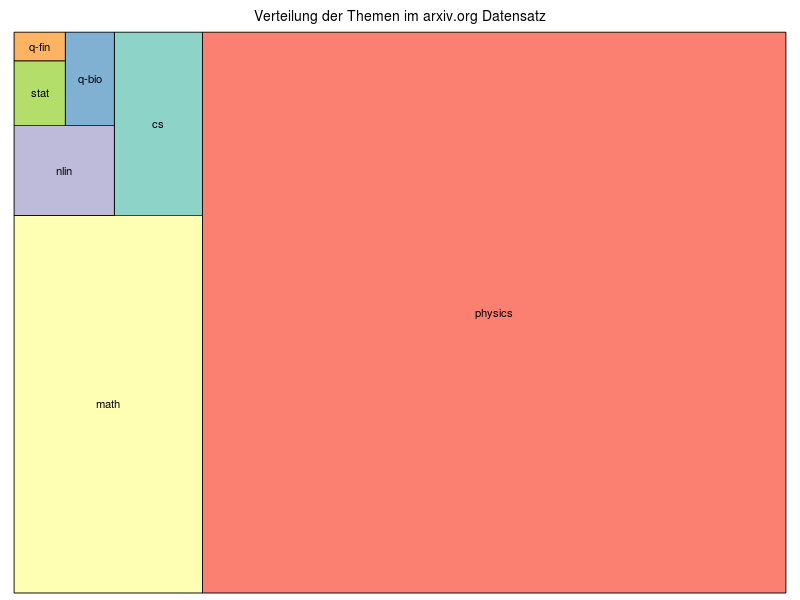
\includegraphics[scale=0.35]{../../visual/treeParent.png}
	%\end{center}
%\end{frame}
%\begin{frame}
	%\frametitle{Aufschlüsselung von physics}
	%\begin{center}
		%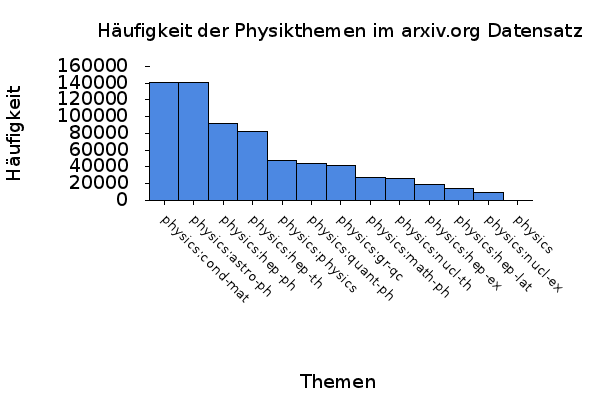
\includegraphics[scale=0.45]{../../visual/setSpecFreq.png}
	%\end{center}
%\end{frame}
%\begin{frame}
	%\frametitle{Häufigkeit von Themen pro Publikation}
	%\begin{columns}
		%\column{.5\textwidth}
    %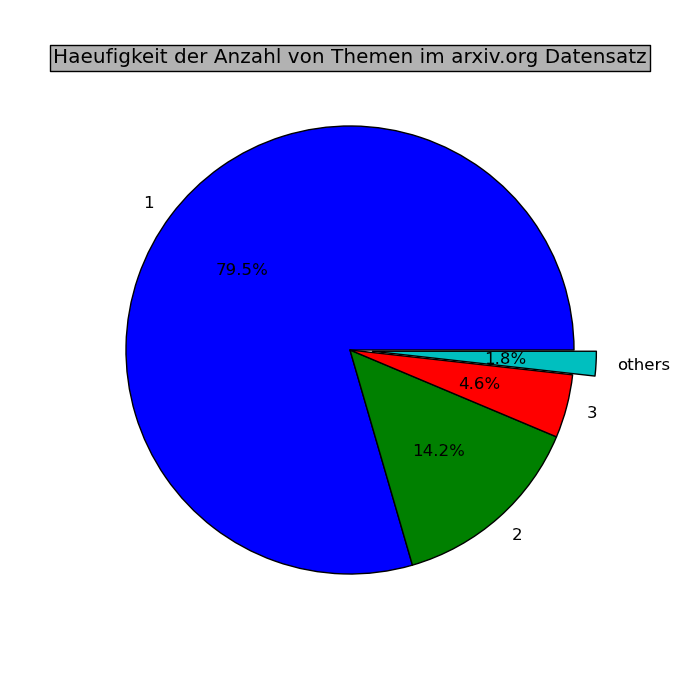
\includegraphics[scale=0.35]{../../visual/piechart.png}
		%\column{.5\textwidth}
    %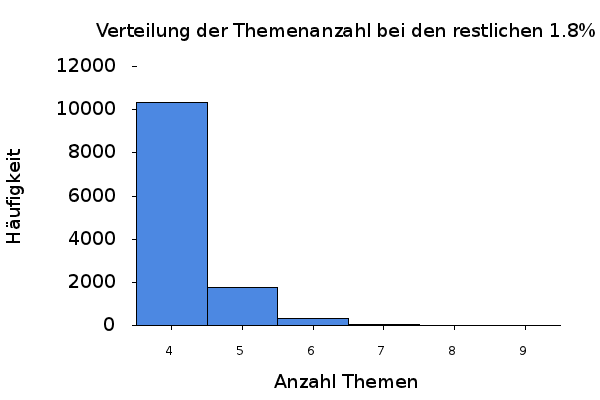
\includegraphics[scale=0.25]{../../visual/pieSubplot.png}
	%\end{columns}
%\end{frame}
%\begin{frame}
	%\frametitle{Was sind Assoziationsregeln?}
	%\begin{itemize}
		%\item bestimmen Korrelation des Auftretes von Mengen
		%\item Regel der Form "Wenn Menge A, dann Menge B"
		%\item Kenngrößen
		%\begin{itemize}
			%\item Support - relative Häufigkeit der Menge in den Daten
			 %\item Konfidenz - Häufikeit des gemeinsames Auftretens von A und B, unter der Bedingung das A auftritt
			 %\item Lift - Bedeutung der Regel
	%\end{itemize}
	%\end{itemize}
%\end{frame}
%\begin{frame}
	%\frametitle{Assoziationsregeln - aller Themen}
	%\begin{center}
	%\begin{table}
	%\rowcolors[]{1}{blue!20}{blue!10}
	%\begin{tabular}{rccc}
		%\tiny\textbf{Regel} &\tiny \textbf{Support} &\tiny \textbf{Konfidenz} & \tiny \textbf{Lift}\\
		%\hline
		%\tiny math $\implies$ stat & \tiny 0.6\% &\tiny 64\% &\tiny 3.0  \\
		%\tiny physics:math-ph $\implies$ math &\tiny 3.8 \% &\tiny 100\% &\tiny 4.7 \\
		%\tiny physics:hep-th, physics:math-ph  $\implies$ math &\tiny 0.9 \% &\tiny 100\% &\tiny 4.7 \\
		%\tiny math, physics:hep-th  $\implies$ physics:math-ph  &\tiny 0.9 \% &\tiny 63\% &\tiny 16.3 \\
		%\tiny physics:gr-qc, physics:hep-th $\implies$ physics:hep-th &\tiny 0.6 \% &\tiny 72 \% &\tiny 6.1 \\
		%\tiny physics:gr-qc, physics:hep-th $\implies$ physics:astro-ph &\tiny 0.6 \% &\tiny 70 \% &\tiny 3.5 \\
		%\tiny physics:gr-qc, physics:astro-ph $\implies$ physics:hep-th &\tiny 0.9 \% &\tiny 50 \%  &\tiny 4.3 \\
		%\tiny physics:astro-ph, physics:hep-th $\implies$ physics:gr-qc  &\tiny 0.9 \% &\tiny 74 \% &\tiny 12.4 \\
	%\end{tabular}
	 %\caption*{Support: 0.5 \% und Konfidenz 50 \%}
	%\end{table}
	%\end{center}
%\end{frame}
%\begin{frame}
	%\frametitle{Assoziationsregeln - Oberthemen}
	%\begin{center}
	%\begin{table}
	%\rowcolors[]{1}{blue!20}{blue!10}
	%\begin{tabular}{rccc}
		%\tiny\textbf{Regel} &\tiny \textbf{Support} &\tiny \textbf{Konfidenz} & \tiny \textbf{Lift}\\
		%\hline
		%\tiny  $\emptyset \implies$ physics & \tiny 78\% &\tiny 78\% &\tiny 1.0  \\
		%\tiny stat $\implies$ math  &\tiny 0.6 \% &\tiny 63 \% &\tiny 3.0 \\
		%\tiny nlin $\implies$ physics  &\tiny 1.3 \% &\tiny 50 \% &\tiny 0.64 \\
		%\tiny math, nlin $\implies$ physics  &\tiny 0.4 \% &\tiny 83 \% &\tiny 1.1 \\
	%\end{tabular}
	 %\caption*{Support: 0.1 \% und Konfidenz 50 \%}
	%\end{table}
	%\end{center}
%\end{frame}
%\begin{frame}
	%\frametitle{Probleme}
	%\begin{itemize}
		%\item mehrere Datumsangaben
		%\item Themen in Metadaten nicht eindeutig
		%\begin{itemize}
			%\item unterschiedliche Kategorisierungen
			%\item auch in einem Eintrag
		%\end{itemize}
		%\item Themenbereiche nachzuschlagen ist aufwendig
	%\end{itemize}
%\end{frame}
%\begin{frame}
	%\frametitle{Weitere Analysen}
	%\begin{itemize}
		%\item Aufschlüsselung der Themenbereiche
		%\item Regeln für die Unterthemen
		%\item Algorithmus implementieren?
			%\begin{itemize}
				%\item AIS-Algorithmnus
				%\item Apriori-Algorithmus 
				%\item FPGrowth 
			%\end{itemize}
		%\item Entwicklung in Abhängigkeit von der Zeit
	%\end{itemize}
%\end{frame}
\end{document}
